\documentclass[12pt, reqno]{amsart}
%%packages (not all immediately neccessary)
\usepackage[latin1]{inputenc}
\usepackage{latexsym}
\usepackage{amsfonts}
\usepackage{amsmath,amssymb}
\usepackage{setspace}
\usepackage{graphicx}
\usepackage{fullpage}
\usepackage{caption}
\usepackage{listings}
\usepackage{xcolor}
\usepackage{url}

\lstset{
    language=Python,
    backgroundcolor=\color{white},
    basicstyle=\ttfamily\small,
    breaklines=true,
    columns=flexible,
    frame=single,
    keepspaces=true,
    keywordstyle=\color{blue},
    commentstyle=\color{gray}\itshape,
    stringstyle=\color{red},
    numbers=left,
    numberstyle=\tiny\color{gray},
    stepnumber=1,
    numbersep=5pt,
    showstringspaces=false,
    xleftmargin=20pt,
    xrightmargin=20pt,
    aboveskip=10pt,
    belowskip=10pt,
    numbers=none
}
%Start of paper
\begin{document}
\title{Numerical Approaches to Solving the Heat Equation}
\author{Andrew Shea}

%Abstract start (\renew makes heading bold)
\renewcommand{\abstractname}{\textbf{Abstract}}
\begin{abstract}
This paper will demonstrate various ways to solve partial differential equations, while highlighting how traditional methods compare to using a neural network based approach. To maintain simplicity and focus on the methods themselves, they will only be implemented on the heat equation. These methods are the Crank-Nicholson method, a Physics-Informed Neural Network (PINN), and an analytical computation. The results of each method will then be observed, measuring data such as accuracy, time required to approximate solutions, and how parameters affect each method.
\end{abstract}
\maketitle


%Start of non-title related sections
\doublespacing
\section{Introduction}
The heat equation is a fundamental partial differential equation (PDE) that mathematically models how heat moves through objects as time passes. It is believed to have first been derived by Joseph Fourier around the year 1822, and was the catalyst for the widespread adoption of Fourier Analysis, a highly applicable concept that is still used in various fields today. Since the heat equation describes the diffusion of heat through a medium, it falls under a broader type of PDE with applications where the concept of diffusivity is present. This concept of a diffusivity PDE was gradually explored and published throughout the 1800's most notably from Adolf Fick (Diffusion in Fluids) and Albert Einstein (Brownian Motion). While the basic heat equation is well understood and has been solved for general solutions, slightly tweaking the equation to account for non-linear or stochastic variables can drastically increase the complexity of it. As a result of this, many of these such cases are not solved analytically but are approximated using various numerical methods. One highly common numerical approach used on the heat equation specifically is the Crank-Nicholson method, a specific type of finite difference method. This is the method of choice because it is unconditionally stable and accurate to the 2nd order in both space and time, making it a well rounded approach to the heat equation. So if numerical approaches are the solution to solving complex diffusivity problems, are Physics-Informed Neural Networks (PINNs) really necessary? The answer to this is yes for two main reasons, the first being that PINNs have the potential to work faster and more accurately than our current numerical methods. The second reason is that while numerical approaches have their fair share of application, there are still instances where the physics of the real world is simply too unstable or computationally expensive to solve numerically. By the end of this paper, the potential of PINNs will be apparent by demonstrating how neural networks can solve PDEs on a simple level, and how their capabilities can be scaled. Hence solving complex partial, and stochastic differential equations in mathematical fields such as engineering, finance, biology, physics and even meteorology.
\textbf{}
\section{An Analytical Approach to the Heat Equation}

%Introduction to the heat equation
\subsection{The Heat Equation in 1-Dimension}
The heat equation in one-dimension is a uniform rod with length L and is given below
\cite{1}.
\begin{equation}\frac{\partial{u}(x,t)}{\partial{t}} = k\frac{\partial^2u(x,t)}{\partial{x^2}}
\end{equation}

\begin{equation} 
u(0,t) = T_0\quad and \quad u(L,t) = T_1
\end{equation}

\begin{equation}
u(x,0) = f(x)
\end{equation}In (1) k is treated as a constant that describes how quickly heat spreads through your material, this is known as the diffusivity constant. Line (2) shows how boundary conditions are expressed, with the temperatures at each end of the domain being $T_0$ and $T_1$. Line (3) shows how initial conditions are expressed, with f(x) being the intital temperature distribution at $t = 0$

\subsection{Solving for an analytical solution}
In this section the heat equation from above will be broken down and solved to find a general solution for homogeneous boundary conditions, meaning the temperature is equal to 0 at both ends. As well as the initial condition $u(x,0) = sin(\pi x)$. The length of our rod L will also be equal to 1.
\subsubsection{Separation of Variables}
Our first step in deriving a general solution for this problem is separating the x and t variables and assuming them to take the following form in our solution. We will then take the necessary partial derivatives of $u(x,t)$ to substitute into our heat equation.
\begin{equation*}
u(x,t) = \phi(x)G(t)
\end{equation*}

\begin{equation}
 \frac{\partial{u(x,t)}}{\partial{t}}= \frac{\partial}{\partial{t}}[\phi(x)G(t)] = \phi(x)\frac{dG(t)}{dt}
\end{equation}

\begin{equation}
\frac{\partial^2{u(x,t)}}{\partial{x^2}} = \frac{\partial^2}{\partial{x^2}}[\phi(x)G(t)] = G(t)\frac{d^2\phi(x)}{dx^2}
\end{equation}
\begin{center}Substituting (4) and (5) into the heat equation (1) yields the following
\begin{equation*}
\phi(x)\frac{dG(t)}{dt} = kG(t)\frac{d^2\phi(x)}{dx^2}
\end{equation*}
We will now fully separate each variable, allowing us to let each side of our equation be equal to the same constant, $-\lambda$, resulting in 2 Ordinary Differential Equations.
\begin{equation*}
\frac{1}{kG(t)}\frac{dG(t)}{dt} = \frac{1}{\phi(x)}\frac{d^2\phi(x)}{dx^2}
\end{equation*}
\begin{equation*}
\frac{1}{kG(t)}\frac{dG(t)}{dt} = -\lambda \quad and \quad \frac{1}{\phi(x)}\frac{d^2\phi(x)}{dx^2} = -\lambda
\end{equation*}
\end{center}
\subsubsection{The Space (x) problem }After multiplying both sides of our space ODE by $\phi(x)$ we are left with the common Second-Order ODE $\frac{d^2\phi(x)}{dx^2} = -\lambda\phi(x)$. This ODE's solutions vary depending on the sign of $\lambda$. We will only work out cases $\lambda > 0$ and $\lambda = 0$; cases $\lambda < 0$ and $\lambda$ being imaginary will be left out, as they both lead to trivial solutions ($\phi(x) = 0$) but require much longer explanations to show. \cite{1}

\begin{equation*}
For\ \lambda > 0: \phi(x) = Asin(\sqrt{\lambda}x)\ + Bcos(\sqrt{\lambda}x)\quad\quad
\end{equation*}
\begin{equation*}
    For\  \lambda = 0: \phi(x) = Ax + B
\end{equation*}
%\begin{center}
We can now apply our Boundary conditions to solve for $\lambda$. Applying our boundary conditions to the $\lambda = 0$ solution only gives trivial solutions, therefore we must apply our boundary conditions to the solution for $\lambda > 0$.
%\end{center}
\begin{equation*}
\phi(x) = Asin(\sqrt{\lambda}x) + Bcos(\sqrt{\lambda}x)
\end{equation*}
From our BC: $\phi(0) = 0$ we get
\begin{equation*}
0 = Asin(\sqrt{\lambda}0) + Bcos(\sqrt{\lambda}0)] = B:
\quad \quad B = 0
\end{equation*}
\begin{equation*}
Now, \phi(x) = Asin(\sqrt{\lambda}x)
\end{equation*}
After using our 2nd BC: $\phi(1) = 0$, and knowing A,L and $\lambda$ cannot = 0 we have
\begin{equation*}
\lambda = (n\pi)^2
\end{equation*}
and our general solution for our space problem follows
\begin{equation*}
\phi_n(x) = A_nsin(n\pi x)
\end{equation*}

\subsubsection{The Time (t) problem}Going back to line (6) we can multiply both sides of our t-problem by $kG(t)$ to get the following ODE.
\begin{equation*}
\frac{dG(t)}{dt} = -\lambda kG(t)
\end{equation*}
The solution for this ODE is quite simple, plugging out $(n\pi)^2$ in for $\lambda$
\begin{equation*}
G(t) = C_ne^{(n\pi)^2kt}
\end{equation*}
\subsubsection{Completing the general solution}
Now that the time and space problem have both been solved, we can now multiply them together as intended in the original $u(x,t) = \phi(x)G(t)$ solution. To get a general solution, we sum over all possible values of n from our eigenvalue.
\begin{equation*}
u(x,t) = \sum_{n=0}^{\infty}A_nsin(n\pi x)e^{-(n\pi)^2kt}
\end{equation*}
Now we apply our initial condition $u(x,0) = sin(\pi x)$
\begin{equation*}
sin(\pi x) = \sum_{n=0}^{\infty}A_nsin(n\pi x)
\end{equation*}
We now have a Fourier series for $sin(\pi x)$ allowing us to determine $A_n$ as
\[
A_n = 
\begin{cases}
A_1 =1 \\
A_n = 0 & \text{if } n \neq 1 \\
\end{cases}\]
Since $A_1 = 1$ and all other $A_n = 0$, the summation reduces to our single initial condition term. We can now express our final solution that satisfies the Heat Equation, Boundary conditions, and Initial conditionas as
\begin{equation*}
u(x,t) = sin(\pi x)e^{-k\pi^2 t}
\end{equation*}

\section{Solving the Heat Equation Numerically}
\subsection{Choosing a Numerical Method}
There are many different types of numerical methods that can be used to solve the Heat Equation Numerically. Such as Forward Euler, Backwards Euler, Crank-Nicholson, Runge-Kutta, ADI (Alternating Direction Implicit), and Finite Element methods \cite{2}. Overall, each of these methods have their strengths and weaknesses, while also being most effective in different situations. After evaluating each of these methods, I decided to choose the Crank-Nicholson method as my numerical method of implementation. I chose this method because it blends the Forwards and Backwards Euler Methods by averaging the two. It is also unconditionally stable for linear PDE's such as the heat equation and maintains second-order accuracy in both space and time \cite{3}. Overall, the Crank-Nicholson method is a good compromise between efficiency and accuracy, and works particularly well for the problem I have chosen.
\subsection{Deriving the Crank-Nicholson Method}
In this section we will cover the entire process of deriving a scheme for our Crank-Nicholson method, from discretizing our domain to getting an equation to represent our approximated solution of the heat equation. We will be approximating the same problem posed in our analytical solution, shown below

\begin{equation*}\frac{\partial{u}(x,t)}{\partial{t}} = k\frac{\partial^2u(x,t)}{\partial{x^2}}
\end{equation*}

\begin{equation*} 
u(0,t) = 0\quad and \quad u(1,t) = 0
\end{equation*}

\begin{equation*}
\frac{\partial{u}}{\partial{x}}(x,0) = sin(\pi x)
\end{equation*}

\subsubsection{Discretizing the domain}
Since computers only handle discrete data, the first step in any numerical method is turning our continuous time and space domains into a mesh, or grid of discrete points. We will do this by defining our time and space grid below
\[
Space\:Grid:\:x_i = i\Delta x , \:for\ i = 0,1,2,3...N
\]
\[
Time\:Grid: \: t^n = n\Delta t,\: for \: n = 0,1,2,3...T
\]
\[
This \:gives:\: u_i^n \approx u(x_i,t^n) \: as \: an \: approximation \: of\: u(x,t)
\]
\subsubsection{Approximating terms}
To get an approximation scheme for our PDE, we must first approximate each term in our Heat Equation. Starting with a centered difference approximation for the time derivative from the left side of our equation
\begin{equation}
\frac{\partial u}{\partial t}(x_i, t^{n+\frac{1}{2}}) \approx \frac{u_i^{n+1} - u_i^n}{\Delta t}
\end{equation}
Next, our spatial derivative from the right side of our PDE will be approximated by taking the average of two centered difference methods at time steps $n$ and $n + 1$, to get $n + \frac{1}{2 }$
\begin{equation}
\frac{\partial^2 u}{\partial x^2}(x_i, t^{n + \frac{1}{2}}) \approx \frac{1}{2} \left( \frac{u_{i+1}^n - 2u_i^n + u_{i - 1}^{n}}{(\Delta x)^2} + \frac{u_{i+1}^{n + 1} -2u_i^{n + 1} + u_{i - 1}^{n + 1}}{(\Delta x)^2}         \right)
\end{equation}
\subsubsection{Completing our Scheme}
Now that we have approximated each term in our PDE, we can substitute equations (6) and (7) into our PDE
\begin{equation*}
\frac{u_i^{n+1} - u_i^n}{\Delta t} = k \cdot \frac{1}{2} \left( 
\frac{u_{i+1}^n - 2u_i^n + u_{i-1}^n}{(\Delta x)^2} + 
\frac{u_{i+1}^{n+1} - 2u_i^{n+1} + u_{i-1}^{n+1}}{(\Delta x)^2} 
\right)
\end{equation*}
Next we can factor $(\Delta x)^2$ out in our right side, multiply both sides by $\Delta t$  and simplify our equation by introducing a constant, $s = \frac{k\Delta t}{(\Delta x)^2}$
\begin{equation*}
u_i^{n+1} - u_i^n = \frac{s}{2}\left( 
u_{i+1}^n - 2u_i^n + u_{i-1}^n + 
u_{i+1}^{n+1} - 2u_i^{n+1} + u_{i-1}^{n+1}
\right)
\end{equation*}
Lastly, all forward time step terms, or $n + 1$ terms, will be rearranged to left side of the equation, and all current time step, or $n$ terms will be moved to the right

\begin{equation*}
u_i^{n+1} - \frac{s}{2}\left(u_{i+1}^{n+1} - 2u_i^{n+1} + u_{i-1}^{n+1}\right)
= u_i^n + \frac{s}{2}\left(u_{i+1}^{n} - 2u_i^{n} + u_{i-1}^{n}\right)
\end{equation*}
Furthermore, the term $\frac{s}{2}$ can be distributed on each side of our equation. Then after combining like terms where necessary, the final result for our update equation is as follows
\begin{equation*}
-\frac{s}{2}u_{i-1}^{n+1} + (1+s)u_i^{n+1}-\frac{s}{2}u_{i+1}^{n+1} = \frac{s}{2}u_{i - 1}^n + (1 - s)u_i^n+\frac{s}{2}u_{i+1}^n
\end{equation*}
\subsubsection{Matrix Formulation and Solving the Linear System}
Our final update equation from above can be written in matrix-vector form as a linear system. Define a vector $\mathbf{u}^n = [u_1^n, u_2^n, ..., u_{i-1}^n]^T$ that holds the approximate values at the current time step, except for the boundaries, since we already know those solutions \cite{3}. We can represent the Crank-Nicholson scheme in the form:

\[
A \mathbf{u}^{n+1} = B \mathbf{u}^{n}
\]

Where $A$ and $B$ are $(N-1) \times (N-1)$ tridiagonal matrices. The matrix $A$ represents the left-hand side coefficients (time step $n+1$), and $B$ represents the right-hand side coefficients (time step $n$). The entries of these matrices are defined as:

\[
A = \begin{bmatrix}
1 + s & -\frac{s}{2} & 0 & \cdots & 0 \\
-\frac{s}{2} & 1 + s & -\frac{s}{2} & \cdots & 0 \\
0 & -\frac{s}{2} & 1 + s & \cdots & 0 \\
\vdots & \vdots & \vdots & \ddots & -\frac{s}{2} \\
0 & 0 & 0 & -\frac{s}{2} & 1 + s
\end{bmatrix}
\quad
B = \begin{bmatrix}
1 - s & \frac{s}{2} & 0 & \cdots & 0 \\
\frac{s}{2} & 1 - s & \frac{s}{2} & \cdots & 0 \\
0 & \frac{s}{2} & 1 - s & \cdots & 0 \\
\vdots & \vdots & \vdots & \ddots & \frac{s}{2} \\
0 & 0 & 0 & \frac{s}{2} & 1 - s
\end{bmatrix}
\]

At each time step, we compute the new solution $\mathbf{u}^{n+1}$ by solving the linear system:

\[
\mathbf{u}^{n+1} = A^{-1} B \mathbf{u}^n
\]

However, rather than explicitly computing the inverse of $A$, we can implement efficient algorithms such as the Thomas algorithm (specialized for tridiagonal systems) to solve $A \mathbf{u}^{n+1} = B \mathbf{u}^n$ directly at each time step \cite{2}. Furthermore, matrix $A$ is Symmetric Positive Definite ensuring numerical stability when solving this system \cite{3}. This formulation provides guaranteed stable and accurate way to advance the numerical solution in time using the Crank-Nicholson method.



\subsection{Implementation of the Crank-Nicholson Scheme}
Now that we have thoroughly derived our numerical method we can go over the implementation of it.
\subsubsection{Matrix Assembly}
The Crank-Nicholson scheme results in a linear system of the form $A \mathbf{u}^{n+1} = B \mathbf{u}^n$ at each time step. Both $A$ and $B$ are tridiagonal matrices that remain constant over all time steps, so we compute them once before the time-stepping loop begins. The python snippet below displays how matrices $A$ and $B$ were initialized as well as how the boundary conditions were set as well.
\begin{lstlisting}[language=Python, title=Matrix Construction]
# === Construct Matrix A
A = np.zeros((3, Nx))
A[0, 1:-1] = -s / 2
A[1, 1:-1] = 1 + s
A[2, 1:-1] = -s / 2
# Dirichlet BCs: keep u[0] and u[-1] fixed at 0
A[1, 0] = 1.0
A[1, -1] = 1.0
A[0, 0] = 0.0
A[2, -1] = 0.0
# Matrix B
B = np.eye(Nx) * (1 - s)
B += np.diag([s / 2] * (Nx - 1), k=1)
B += np.diag([s / 2] * (Nx - 1), k=-1)  
B[0, :] = 0
B[0, 0] = 1
B[-1, :] = 0
B[-1, -1] = 1
\end{lstlisting}

\subsubsection{Time Stepping}
Once the matrices and other proper variables are initialized, the time stepping loop shown below can be run to solve all the systems required to approximate the solution.


\begin{lstlisting}[language=Python, title = Time Stepping Loop]
# === Time stepping loop ===
#NOTE: u is initialized at the very beginning with the corresponding intial condition as u = sin(pi*x), the variable Nt is the total number of time steps, initialized as 20,000
for n in range(1, Nt + 1):
    b_ = B @ u
    b_[0] = 0.0     # enforce Dirichlet BC at x=0
    b_[-1] = 0.0    # enforce Dirichlet BC at x=L
    u = solve_banded((1, 1), A, b_)
    u[0] = 0.0      # enforce Dirichlet BC after solve
    u[-1] = 0.0
    solution[n, :] = u
\end{lstlisting}

\subsubsection{Calculating Error and Collecting Data}
After the entire time stepping loop, or in other words the simulation of our heat equation is complete, we can take the data we have approximated and compare it to the analytical solution to collect data and calculate our total error. The code below defines the analytical solution, descretizes it into our numerical domain, then compares it to our approximated solution to get the Max Error, Mean Squared Error, and Mean Average Error

\begin{lstlisting}[language=Python, title = Data Collection and Error Calculation]
# === Analytical solution ===
def exact_solution(x, t, k):
    return np.exp(-np.pi**2 * k * t) * np.sin(np.pi * x)
#Descretize exact solution to match approximation format
t_values = np.linspace(0, T, Nt + 1)
exact_sol = np.array([[exact_solution(x[j], t_values[i], k) for j in range(Nx)] for i in range(Nt + 1)])
#Calculate Error by comparing numerical solution to analytical solution
error = np.abs(solution - exact_sol)
mae = np.mean(error)
mse = np.mean(error**2)
max_error = np.max(error)
\end{lstlisting}

\subsection{Summary of Numerical Approach}
This fully concludes this section on a numerical approach to the Heat Equation. To summarize, we briefly discussed different options, chose the Crank-Nicholson method, derived our method, implemented our derivation, then collected data on it. All collected data will be observed and compared to our other methods at the end, where we will draw conclusions from our work.


\section{Solving the Heat Equation using a Physics Informed Neural Network}
\subsection{Foundations of Physics-Informed Neural Networks}
This section will introduce the basics of neural networks and how they work.
\subsubsection{Architecture of Neural Networks}
Artificial neural networks are computational models inspired the overall structure and functions of biological neurons found in the brain \cite{4}. At the base level neural networks are composed of neurons, or nodes arranged in layers to make up the networks architecture. A typical architecture starts with an input layer, will have one or more hidden layer, and then an output layer. The input layer is where data is entered, the hidden layers are where approximation primarily occurs, and the output layer is responsible for outputting results. Every connection between nodes carries its own weight, and each node applies a transformation to its input using an activation function and a bias \cite{4}. 
\subsubsection{Calculating the transformation}
The transformation calculation is shown below with the following descriptions.
\begin{align*}
z^{(l+1)} &= W^{(l)} x^{(l)} + b^{(l)} \\
x^{(l)} &= \sigma\left(z^{(l)}\right)
\end{align*}
\begin{itemize}
    \item \( z^{(l)} \): The input to the activation function at layer \( l \)
    \item \( x^{(l)} \): The output from layer \( l \) after applying the activation function to \( z^{(l)} \)
    \item \( W^{(l)} \): The weight matrix connecting layer \( l \) to layer \( l+1 \); each entry represents the strength of a connection between neurons.
    \item \( b^{(l)} \): The bias vector added at layer \( l \) before applying the activation function; allows for shifting the activation.
    \item \( \sigma(\cdot) \): The activation function (e.g., ReLU, tanh), applied element-wise.
    \item \( l \): The index of the current layer in a neural network.
\end{itemize}
\subsubsection{The activation function}
The activation function is a key component of the learning process for a neural network. The function is a non-linear mapping between inputs and outputs, allowing the network to learn complex, non-linear patterns in data. If a network didn't have an activation function, then it would simply be a linear transformation of the input data, and it would not be able to learn non-linear relationships \cite{4}. Some basic activation functions are shown below.
\begin{enumerate}
    \item \textbf{ReLU (Rectified Linear Unit):}
    \[
    \text{ReLU}(x) = \max(0, x)
    \]
    \textit{Maps} \( x \in \mathbb{R} \rightarrow [0, \infty) \).  
    \textbf{Use case:} Popular for its simplicity and effectiveness, especially in image-related tasks. Not smooth at \( x = 0 \), so less ideal for PDEs in PINNs.

    \item \textbf{Sigmoid:}
    \[
    \sigma(x) = \frac{1}{1 + e^{-x}}
    \]
    \textit{Maps} \( x \in \mathbb{R} \rightarrow (0, 1) \).  
    \textbf{Use case:} Good for probabilistic outputs and binary classification.

    \item \textbf{Tanh (Hyperbolic Tangent):}
    \[
    \tanh(x) = \frac{e^x - e^{-x}}{e^x + e^{-x}}
    \]
    \textit{Maps} \( x \in \mathbb{R} \rightarrow (-1, 1) \).  
    \textbf{Use case:} Preferred in PINNs due to its smoothness and symmetry around zero. Can also map to negative and positive values if needed.
\end{enumerate}
\subsubsection{The Forward pass and backpropagation}
For a feed forward neural network, the forward pass is the process of a layer taking in an input, transforming it into an output, and passing that output forward to the next layer. The transformation is performed by the method defined above, using weights, biases, and the nonlinear activation function. Once a forward pass is completed through the neural network, we use backpropagation. This is an algorithm used to compute gradients of the loss with respect to each weight and bias in the network \cite{4}. This process is made possible by autograd, or automatic differentiation, which constructs a computational graph during the forward pass and traverses backwards through the network to calculate derivatives. These gradients are then used by a predefined optimizer, with a specified learning rate that goes into the network and updates weights and biases to minimize loss \cite{4}. The learning rate is a value that the optimizer uses to decide how drastic of updates to make to the weights and biases, the lower the learning rate the smaller updates it will make.
\subsection{From Neural Networks to PINNs}
As defined above, traditional neural networks excel at fitting data, not necessarily to respect physical laws. Physics Informed Neural Networks fix this by embedding the governing equations of a physical system, such as a PDE, into its training process.
\subsubsection{PINNs vs Traditional Neural Networks}
The core concept that sets PINNs apart from Neural Networks is how the loss function is designed. In traditional networks, the loss is a measure of difference between predicted outputs and already obtained data. When approximating a PINN, we don't already have the solution, or in this case the data needed to calculate the loss. Therefore we must incorporate the PDE itself along with any other necessary conditions into the loss function. This allows the network to learn a solution to the PDE and its conditions, rather than just trying to fit data.
\subsubsection{PDEs in the loss function}
In order to put the heat equation directly into the loss function we first rearrange it to the following form.
\begin{equation*}
0 = \frac{\partial u}{\partial t} - k\frac{\partial^2u}{\partial x^2}
\end{equation*}
Next we can define some function $f(x,t)$ where
\begin{equation*}
f(x,t) = \frac{\partial u}{\partial t} - k\frac{\partial^2u}{\partial x^2}
\end{equation*}
By using this in our loss function, we know that $f(x,t)$ will be closer to 0 the more accurate our network is. Therefore we can use this as a training standard for our network, and penalize our network the further $f(x,t)$ is from 0. Furthermore, rather than just evaluating $|f(x,t)|$, we can calculate the Mean Squared Error for all predicted points to ensure smooth gradients and to give larger penalties more effectively.
\subsubsection{Boundary and Initial Conditions in the loss function}
In the same way the PDE is incorporated into the loss function, the boundary and initial conditions are also considered as well. The mean squared error is also computed for the initial and boundary loss for the same reasons as above. Finally, the PDE loss, initial condition loss, and boundary condition loss, can all be combined together to get one total loss function for the network to train on.
\subsubsection{Why Autograd is so important}
Autograd is essential to making PINNs work. The concept of autograd introduced previously is what allows the model to compute derivatives inside of our loss function. Without autograd, computing the necessary derivatives such as $\frac{\partial u}{\partial t}$ and $\frac{\partial ^2 u}{\partial x^2}$, which are central to the loss function, would be a highly manual and prone to errors. Autograd is implemented and computed internally in libraries such as PyTorch and TensorFlow.
\subsection{Pros and Cons of PINNs}
\subsubsection{Pros of PINNs}
One of the most significant and important qualities of PINNs is that they are mesh free. Meaning that they don't require the creation of a discrete mesh or grid that was required before implementing a numerical method. Numerical methods often rely on carefully chosen sizes for these meshes, can be computationally expensive. Furthermore, meshes do not scale well with dimensions either, as the number of points in a mesh grows exponentially with the number of dimensions.
\subsubsection{Cons of PINNs}
The biggest challenges PINNs face is their performance is solely based on the skill level of the person implementing it. The accuracy of PINNs can be highly sensitive to the overall structure of the network, such as layers used, amount of nodes per layer, and activation functions used. While also being just as sensitive to hyperparameter used such as the optimizer, learning rate, batch size, and number of epochs the network trains on.
\subsection{Implementing a PINN for the Heat Equation}
This section will go over how I implemented a PINN to solve the heat equation problem from the previous methods, as shown below
\begin{equation*}\frac{\partial{u}(x,t)}{\partial{t}} = k\frac{\partial^2u(x,t)}{\partial{x^2}}
\end{equation*}

\begin{equation*} 
u(0,t) = 0\quad and \quad u(1,t) = 0
\end{equation*}

\begin{equation*}
\frac{\partial{u}}{\partial{x}}(x,0) = sin(\pi x)
\end{equation*}

\subsubsection{Network Architecture}
In my implementation, the structure of my network consisted of an input layer with two nodes, three hidden layers with forty nodes each, and an output layer with one node. The input layer had two nodes, one to take in time values, and the other to take in space values from the function $u(x,t)$. I chose three hidden layers with forty nodes each because it offered a good balance between expressive power and computational efficiency. The output layer only had one node, which returned the predicted temperature corresponding to the input pair $(x,t)$. The hyperbolic tangent (tanh) activation function was used in each hidden layer due to its smoothness, differentiability, and its output range of (-1,1), which helps center data and stabilize gradient-based optimization. Lastly, the weights were initialized using Xavier initialization, which gives the weights a uniform distribution based on the number of input and output nodes in each layer. This method will help mitigate the risk of gradients vanishing or exploding in the training process \cite{4}. A snippet of my initialization method can be seen below, where I used the PyTorch framework to initialize the network using the torch module.
\begin{lstlisting}[language=Python, title = PINN Initialization]
class Net1D(nn.Module):
    def init(self, input_size, hidden_size, output_size):
        super(Net1D, self).init()
        self.hidden = nn.Sequential(
            nn.Linear(input_size, hidden_size),
            nn.Tanh(),
            nn.Linear(hidden_size, hidden_size),
            nn.Tanh(),
            nn.Linear(hidden_size, output_size)
        )
        self.apply(self.xavier_init)

    def forward(self, x):
        return self.hidden(x)

    def xavier_init(self, m):
        if isinstance(m, nn.Linear):
            nn.init.xavier_normal_(m.weight)
            nn.init.zeros_(m.bias)
\end{lstlisting}
\subsubsection{Loss Function}
Once the network is initialized, the next important step taken was defining the loss function for the network to train on. I computed the PDE loss, Boundary loss, and Initial loss separately. Next I weighted each loss by multiplying them by a determined constant, then summed the weighted calculations together to get a total loss for the network to use in training \cite{5}. The PDE loss was given a weight of 10, while the boundary and initial condition loss each had a weight of 1, prioritizing minimizing PDE loss over condition loss. When calculating each loss, I calculated the MSE for each to penalize the network more for higher error. Autograd was used to calculate the time and spacial derivatives in the PDE loss function, while it was not needed in boundary or initial loss; since there are no derivatives on those formulas \cite{5}. Below is the code snippet where I calculated each loss independently then summed them all together in my return statement.
\begin{lstlisting}[language = Python, title = Loss Calculation Function]
# Compute the full loss
def compute_loss(net, x, t, bc_weight=1.0, ic_weight=1.0, pde_weight=10.0):
    xt = torch.cat([x, t], dim=1).to(device)
    xt.requires_grad = True
    u = net(xt)
    #PDE Loss
    grads = torch.autograd.grad(u, xt, torch.ones_like(u), create_graph=True)[0]
    u_t = grads[:, 1:2]
    u_x = grads[:, 0:1]
    u_xx = torch.autograd.grad(u_x, xt, torch.ones_like(u_x), create_graph=True)[0][:, 0:1]
    pde_loss = ((u_t - k * u_xx) ** 2).mean()
    # Boundary Condition loss
    t_bc = torch.rand(x.shape[0], 1).to(device)
    x0 = torch.zeros_like(t_bc)
    x1 = torch.ones_like(t_bc)
    u0 = net(torch.cat([x0, t_bc], dim=1))
    u1 = net(torch.cat([x1, t_bc], dim=1))
    bc_loss = (u0 ** 2).mean() + (u1 ** 2).mean()
    # Initial Condition loss
    x_ic = torch.rand(x.shape[0], 1).to(device)
    t0 = torch.zeros_like(x_ic)
    u_ic = net(torch.cat([x_ic, t0], dim=1))
    ic_loss = ((u_ic - torch.sin(np.pi * x_ic)) ** 2).mean()
    #total loss 
    total_loss = pde_weight * pde_loss + bc_weight * bc_loss + ic_weight * ic_loss
    return total_loss, pde_loss.item(), bc_loss.item(), ic_loss.item()
\end{lstlisting}
\subsubsection{Training Details}
The last step in creating the PINN was training and running the model. The first step in training is calling the initialization method, passing through the size of each layer to initialize the network. Next I defined which optimizer I would use when performing backpropagation. I chose the Adam optimizer with a learning rate of $lr = .001$, a popular and well rounded choice especially for PINNs. Next I defined how many epochs, or training iterations, I wanted the network to perform. I trained the model on 15,000 epochs, where every epoch the model randomly generated 2,000 points to train on, this is known as the batch size. At the end of training loop, I added a print statement to give updates on the PDE, condition, and total loss every 1,000 epochs. The complete code for this process is shown below. 
\begin{lstlisting}[language = python, title = Training paramaters and loop]
# Training parameters
k = 0.1
net = Net1D(2, 40, 1).to(device)
optimizer = torch.optim.Adam(net.parameters(), lr=1e-3)
epochs = 15000
N_train = 2000
loss_history = []
for epoch in range(1, epochs + 1):
    x = torch.rand(N_train, 1).to(device)
    t = torch.rand(N_train, 1).to(device)

    optimizer.zero_grad()
    loss, pde_l, bc_l, ic_l = compute_loss(net, x, t)
    loss.backward()
    optimizer.step()
    if epoch % 1000 == 0 or epoch == 1:
        print(f"Epoch {epoch}: Loss={loss.item():.6f} | PDE={pde_l:.6f}, BC={bc_l:.6f}, IC={ic_l:.6f}")
        loss_history.append(loss.item())
    
\end{lstlisting}



\section{Results and Data Comparisons}
This section will go over the results from each methods. The numerical method and PINN produced a solution heatmap, that we will compare to a heat map obtained from graphing our analytical solution. Error data and heatmaps were also tracked in the numerical method and PINN, so those figures will be compared here as well.
\subsection{Solutions heatmaps, Error Metrics, and Error Heatmaps}
Below are all figures produced from the implementations. First the Crank-Nicholson solution is compared to the Analytical Solution, then then same comparison is done with the PINN. Afterwards the Error heatmaps for each implementation is shown with their metrics attached to the bottom of each figure.
\newpage
\begin{figure*}
\captionsetup{labelformat = empty}
    \caption{Crank-Nicholson solution vs Analytical Solution}
    \centering
    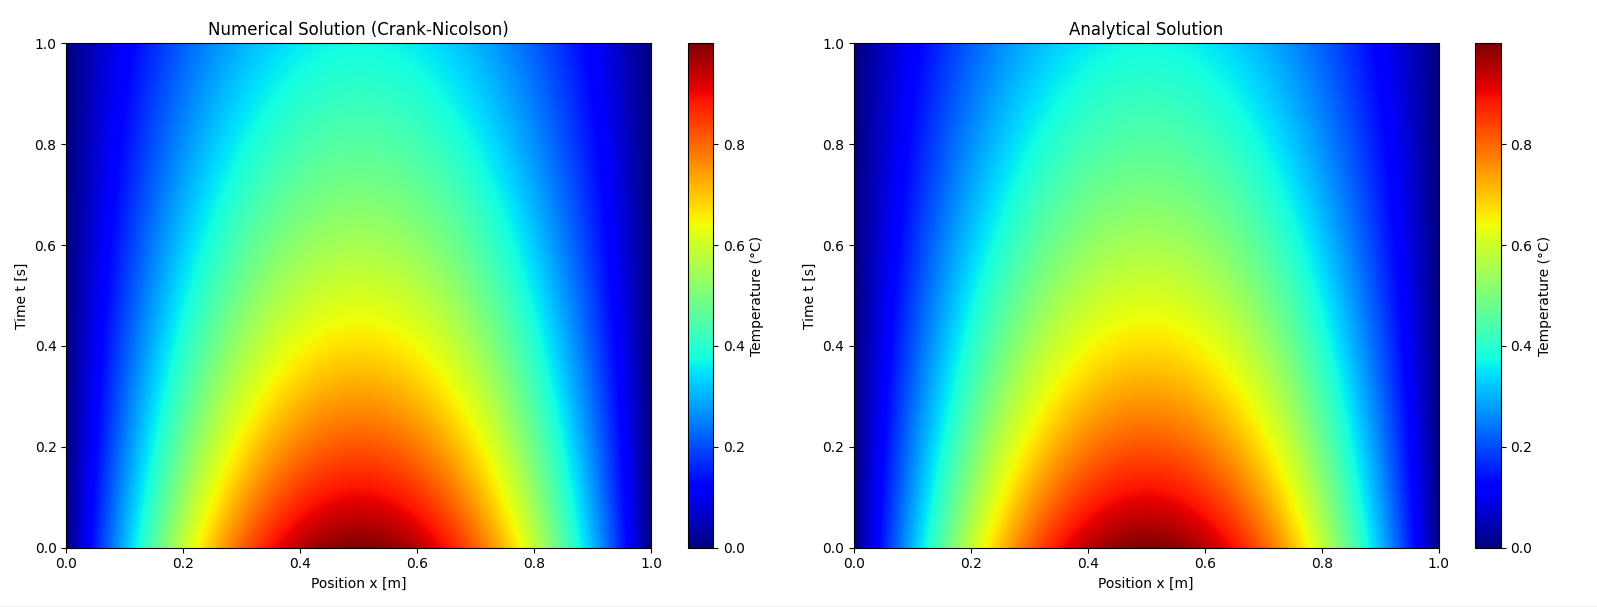
\includegraphics[width=.9\linewidth]{CRANK NICOLSON FINAL.png}
\end{figure*}
\begin{figure*}
\captionsetup{labelformat = empty}
    \caption{Crank-Nicholson solution vs Analytical Solution}
    \centering
    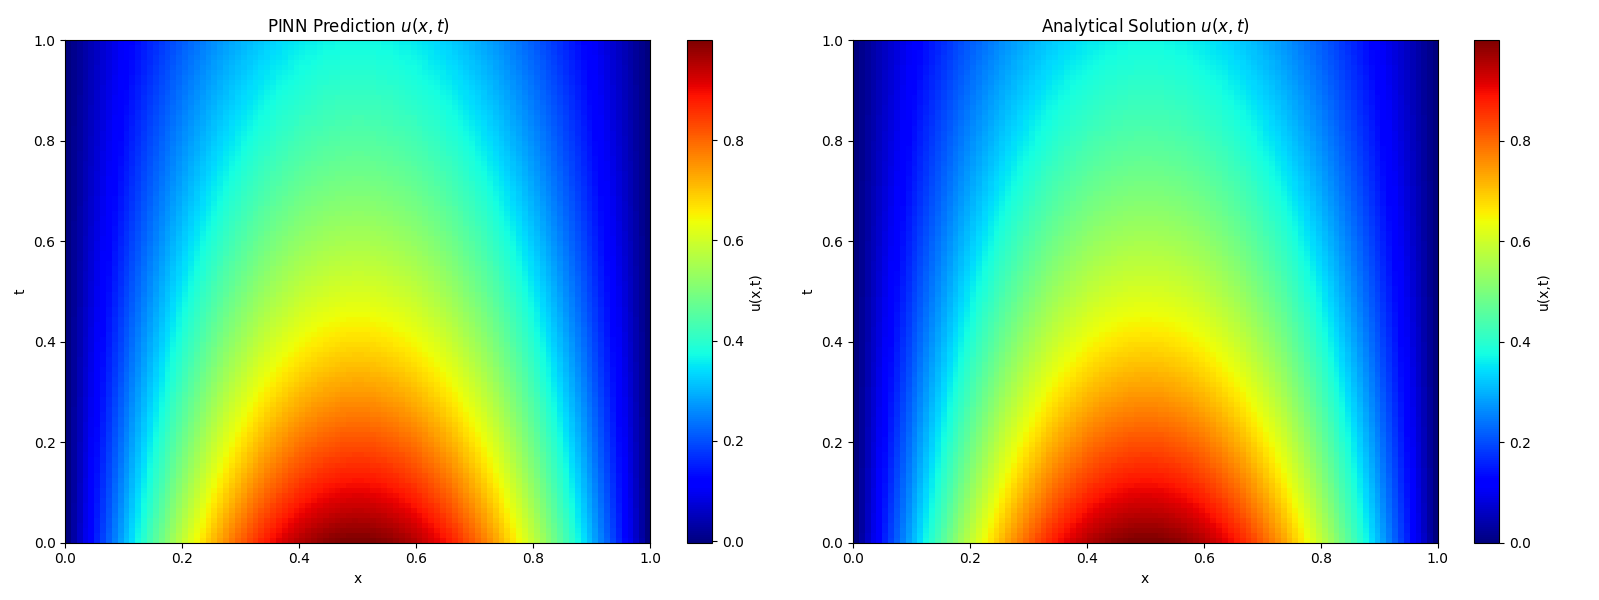
\includegraphics[width=.9\linewidth]{PINN GRAPH FINAL.png}
\end{figure*}
\begin{figure*}
\captionsetup{labelformat = empty}
    \caption{Crank-Nicholson Error vs PINN Error}
    \centering
    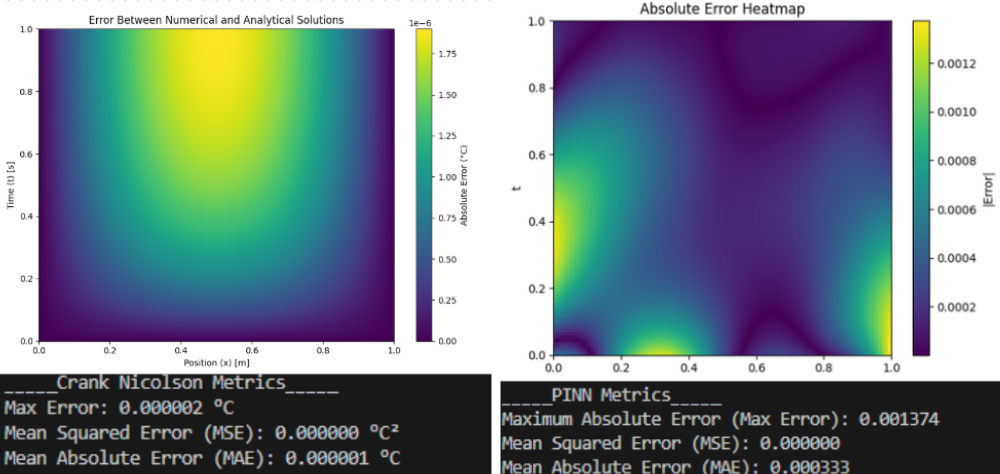
\includegraphics[width=.9\linewidth]{ERROR MAPS.png}
\end{figure*}
\clearpage
\subsection{Observations and Conclusions}
This section will cover conclusions drawn from each figure above.
\subsubsection{Solutions}
As seen in the solutions heatmaps above, both the numerical method and the PINN did a great job at visually approximating the solution, as there are little to no differences in each solutions heatmap.
\subsubsection{Error Metrics}
Since the heatmaps did not show any noticeable difference in the methods, the error data above was collected for each method. The Maximu Error, Mean Squared Error, and Mean Absolute Error was computed for each method. As seen in the figure, the numerical method was more accurate than the PINN. This was somewhat expected before the implementation process, as PINNs advantages are mostly found in complex problems with higher dimensions than 1.
\subsubsection{Error Heatmap}
An immediate conclusion in regards to the error heatmaps can be instantly drawn just from observing the two graphs. On the left, the error from the Crank-Nicholson method is very uniform and is clearly higher further from the domain boundaries, since only interior points were approximated. Furthermore, the error increases over time due to the accumulation and propagation of numerical approximation errors at each time step. On the other hand, the error distribution for the PINN is very randomized and unpredictable. This is attributed to the PINN being trained on randomized points throughout the training process. Since the PINN is trained on completely randomized points, then it will be more accurate around the randomly spaced points it trained on. There are other ways of getting training points than randomization, such as predefining a grid of training points, however randomization is sometimes a key component for generalization in the training process. Furthermore, if a predefined grid were used as a training batch, the PINN begins to enter this territory of only being as accurate as the number of points the grid will contain, which is no different than discretizing the domain for the accuracy of a numerical method. 
\section{Conclusion}
In this work, we defined the heat equation and the problem we would be working on, then proceeded to derive and implement three different solution methods; an analytical solution, numerical method, and Physics-Informed Neural Network. After the implementation of method, solutions were graphed and error data was collected for comparison. As expected, the numerical method performed better than the PINN, primarily because PINNs perform better on more complex problems and in higher dimensions. Overall, the study highlighted the strengths and weaknesses of each method, and gave insight into how PINNs can be used in the future.
\bibliographystyle{plain}
\begin{thebibliography}{10}
\bibitem{1}
R. Haberman.
\newblock {\em Applied Partial Differential Equations with Fourier Series and Boundary Value Problems}.
\newblock 5th ed., Pearson, 2019.

\bibitem{2}
Timothy Sauer.
\newblock {\em Numerical Analysis}, 3rd edition.
\newblock Pearson, 2019.



\bibitem{3}
J. Peterson.
\newblock {\em Crank-Nicolson Scheme}.
\newblock Florida State University, 2017.
\newblock \url{https://people.sc.fsu.edu/~jpeterson/5-CrankNicolson.pdf}.




\bibitem{4}
M. Islam, G. Chen, and S. Jin.
\newblock An overview of neural network.
\newblock {\em American Journal of Neural Networks and Applications}, 5(1):7--11, 2019.
\newblock doi: 10.11648/j.ajnna.20190501.12.


\bibitem{5}
F. Foobot.
\newblock Physics-Informed Neural Networks (PINNs) for Heat Equation.
\newblock {\em Foobot Blog}, 2021.
\newblock \url{https://techblog.foobot.io/ai/deeplearning/physics/pinns-heat-equation.html}.


\end{thebibliography}
\end{document}
